\documentclass{beamer}

\usepackage{pgf, tikz}
\usetikzlibrary{decorations.markings}
\usetikzlibrary{math}

\newcommand{\D}{{\mathrm d}}
\newcommand{\e}{{\mathrm e}}

% to get page number in footer
\addtobeamertemplate{navigation symbols}{}{%
    \usebeamerfont{footline}%
    \usebeamercolor[fg]{footline}%
    \hspace{1em}%
    \insertframenumber/\inserttotalframenumber
}



\begin{document}



% ____________________________________________________________________________
\begin{frame}
\frametitle{Simuler numériquement un plasma...}

Un plasma est un gaz de particules ionisées :

\begin{center}
\begin{tabular}{cc}
\includegraphics[width=0.45\textwidth]{heliosphere.jpg} &
\includegraphics[width=0.45\textwidth]{41467_2018_3548_Fig4_HTML.png} \\
\end{tabular}
\end{center}

$\bullet$ Les particules chargées se déplacent sous l'effet de $\mathbf E$ et $\mathbf B$ \\
$\bullet$ Les champs $\mathbf E$ et $\mathbf B$ évoluent avec les termes source $\rho$ et $\mathbf J$ \\

\begin{center}
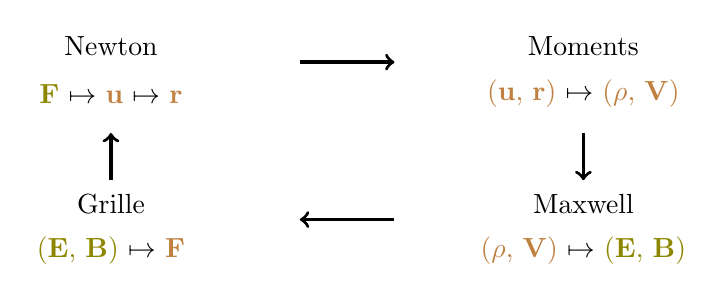
\begin{tikzpicture}[scale=1.0]

\node at ( -3.0, 4.0) {Newton};
\node at ( -3.0, 3.4) {\textcolor{olive}{\textbf{F}} $\mapsto$ \textcolor{brown}{\textbf{u}} $\mapsto$ \textcolor{brown}{\textbf{r}}};

\draw[very thick, ->] ( -0.6, 3.8) -- ( 0.6, 3.8);

\node at (  3.0, 4.0) {Moments};
\node at (  3.0, 3.4) {\textcolor{brown}{(\textbf{u}, \textbf{r})} $\mapsto$ \textcolor{brown}{($\rho$, \textbf{V})}};

\draw[very thick, ->] (  3.0, 2.9) -- ( 3.0, 2.3);

\node at (  3.0, 2.0) {Maxwell};
\node at (  3.0, 1.4) {\textcolor{brown}{($\rho$, \textbf{V})} $\mapsto$ \textcolor{olive}{(\textbf{E}, \textbf{B})}};

\draw[very thick, <-] ( -0.6, 1.8) -- ( 0.6, 1.8);

\node at ( -3.0, 2.0) {Grille};
\node at ( -3.0, 1.4) {\textcolor{olive}{(\textbf{E}, \textbf{B})} $\mapsto$ \textcolor{brown}{\textbf{F}}};

\draw[very thick, <-] ( -3.0, 2.9) -- (-3.0, 2.3);


\end{tikzpicture}

\end{center}

\end{frame}


\end{document}
